\documentclass[../../compsys.tex]{subfiles}
\begin{document}
\raggedbottom
\chapter{L17 - The Link Layer}
\vfill
\textit{Having studied how the network layer routes packets across the Internet, we now examine how individual network segments deliver those packets locally. This brings us to the link layer.}

\section{Fundamentals}

\subsection{Packet Switch Types}

Networks contain two fundamentally different types of packet switches:

\begin{itemize}
    \item \textbf{Link-layer switches}: Operate at physical and link layers, forwarding packets within a single network segment using physical addresses
    \item \textbf{Network-layer switches (routers)}: Operate at physical, link, and network layers, routing packets between different networks using IP addresses
\end{itemize}

\textbf{Terminology:} Throughout this course, ``switch'' refers to link-layer switches, while ``router'' refers to network-layer switches.

\subsection{Scope Comparison: Link vs Network Layer}

The key distinction lies in their operational scope:

\begin{description}
    \item[Network Layer:] Delivers packets \emph{end-to-end across the entire network} (e.g., New York to Tokyo across the Internet)
    \item[Link Layer:] Delivers packets \emph{across a single physical link} (e.g., laptop to wireless access point)
\end{description}

Think of the network layer as the postal service routing mail globally, while the link layer is the local delivery truck carrying mail from the post office to your house.

\subsection{Layer Roles Within IP Subnets}

Consider a single IP subnet---essentially one network segment like your home WiFi:

\begin{center}
    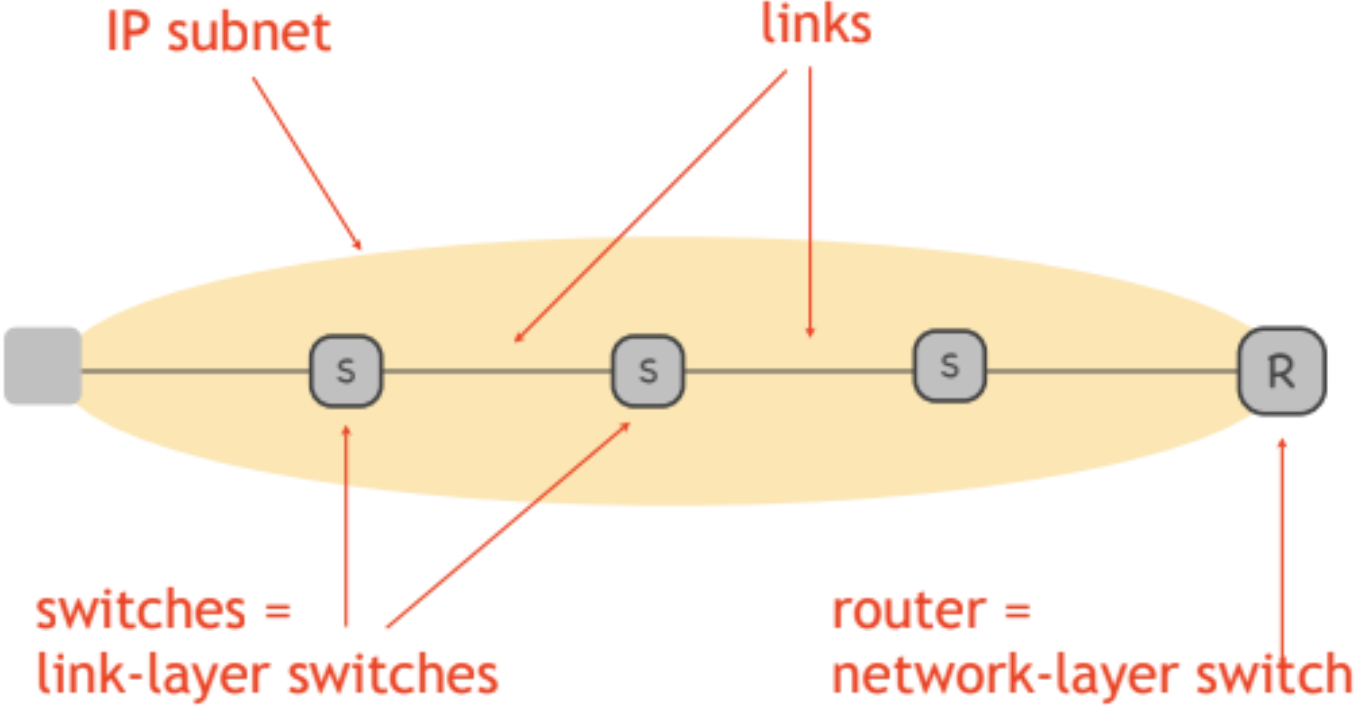
\includegraphics[width=0.5\textwidth]{images/subnet.png}
\end{center}

Within this subnet containing end-systems, boundary routers, and interconnecting switches:

\begin{itemize}
    \item \textbf{Link layer:} Moves packets across individual physical connections (one ``hop'')
    \item \textbf{Network layer:} Moves packets across the entire subnet (multiple hops, e.g., from left computer to router R)
\end{itemize}

\subsection{Internet-Scale Architecture}

Zooming out to the full Internet reveals multiple interconnected IP subnets:

\begin{center}
    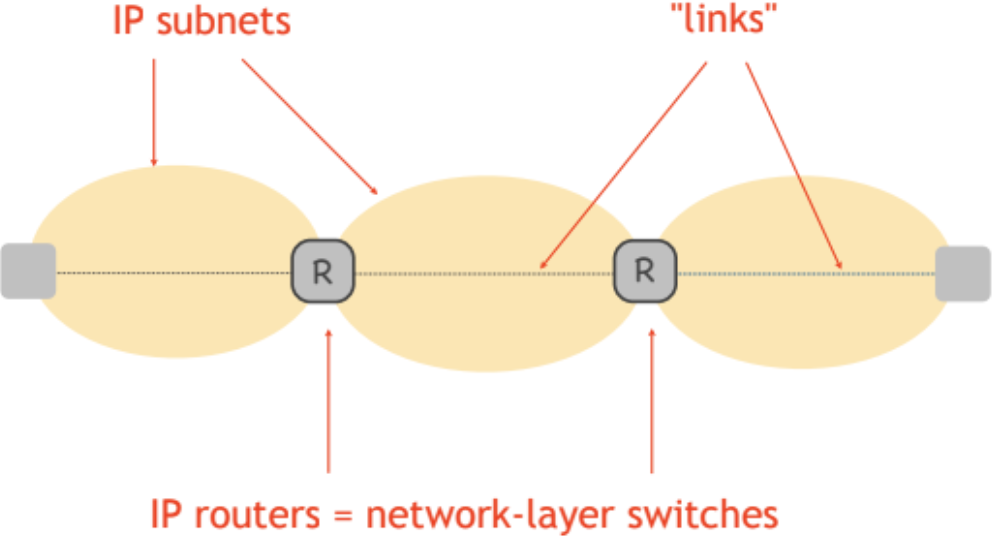
\includegraphics[width=0.5\textwidth]{images/internet-subnets.png}
\end{center}

This layered approach enables Internet scalability:
\begin{itemize}
    \item Network layer handles inter-subnet routing without knowing physical link details
    \item Link layer handles local delivery without understanding global routing
\end{itemize}

Each layer focuses on its specific scope, making the overall system manageable and efficient.

\subsection{Perspective Matters: Two Views of ``Link Layer''}

The term ``link layer'' actually has different meanings depending on your perspective:

\begin{description}
    \item[IP Subnet Perspective:] Link layer moves packets across individual physical links (cable, WiFi connection)
    \item[Internet Perspective:] Link layer moves packets across entire IP subnets (what we call network layer within a subnet)
\end{description}

From the Internet's viewpoint, each IP subnet is just one ``link'' in the larger network. This is why the Internet's ``link layer'' is actually the network layer of individual subnets.

\section{Link-Layer Services}

The link layer (focusing on physical links within subnets) provides several key services:

\subsection{Error Detection}
\begin{itemize}
    \item Receivers detect and drop corrupted packets using checksums
    \item Similar to UDP/TCP error detection but at the physical link level
\end{itemize}

\subsection{Reliable Data Delivery}
\begin{itemize}
    \item Sender/receiver detect corruption and loss, attempting recovery
    \item Uses checksums, acknowledgments, and retransmissions
    \item Typically deployed only on error-prone links (especially wireless)
\end{itemize}

\subsubsection{Why Link-Layer Reliability?}

Since TCP provides end-to-end reliability, why also implement it at the link layer? The answer is \textbf{performance optimization}.

Consider a long network path where one link experiences frequent packet loss:

\textbf{Without link-layer reliability:}
\begin{enumerate}
    \item TCP times out waiting for acknowledgments
    \item Resets congestion window to minimum
    \item Slowly ramps up transmission rate again
    \item Overall throughput drops significantly
\end{enumerate}

\textbf{With link-layer reliability:}
\begin{enumerate}
    \item Link layer locally detects and retransmits lost packets
    \item TCP never sees the packet loss
    \item No TCP timeout or congestion window reset
    \item Maintains higher end-to-end throughput
\end{enumerate}

This local recovery is much faster than end-to-end TCP recovery, especially over long network paths.

\subsection{Medium Access Control (MAC)}
\begin{itemize}
    \item Manages access to shared physical medium (e.g., wireless spectrum)
    \item Detects collisions when multiple devices transmit simultaneously
    \item Implements backoff and retry mechanisms
\end{itemize}

\newpage
\section{Ethernet Networks}

Now let's examine how packets actually move within an IP subnet, focusing on Ethernet---the dominant technology for local area networks.

\subsection{MAC Addresses}

Every network interface in an Ethernet subnet has a unique \textbf{MAC address} (also called Ethernet address or physical address):

\begin{itemize}
    \item \textbf{Format:} 48-bit number, typically written as six hexadecimal bytes
    \item \textbf{Example:} \texttt{5c:f9:38:a4:00:76}
    \item \textbf{Addressing:} Flat (not hierarchical like IP addresses)
    \item \textbf{Scope:} Globally unique but location-independent
\end{itemize}

\subsubsection{Intra-Subnet Communication}

When devices communicate within the same IP subnet, packets carry Ethernet headers containing source and destination MAC addresses:

\begin{center}
\begin{tabular}{|c|c|c|}
\hline
\textbf{Link-layer header} & \textbf{Network header} & \textbf{Data} \\
\hline
src MAC | dst MAC & IP header & Payload \\
\hline
\end{tabular}
\end{center}

For communication between two devices in the same subnet:
\begin{itemize}
    \item \textbf{Source MAC:} Address of the sending device's network interface
    \item \textbf{Destination MAC:} Address of the receiving device's network interface
\end{itemize}

\subsubsection{Inter-Subnet Communication}

When a device sends packets to a different IP subnet, the MAC addressing changes as the packet traverses the local subnet:

\begin{itemize}
    \item \textbf{Source MAC:} Sending device's MAC address
    \item \textbf{Destination MAC:} Border router's MAC address (not the final destination!)
\end{itemize}

\textbf{Key principle:} Within any IP subnet, packets always carry MAC addresses from devices \emph{within that subnet}. The source MAC belongs to whichever device first forwards the packet in this subnet, while the destination MAC belongs to whichever device will receive the packet last in this subnet.

This means MAC addresses change as packets cross subnet boundaries, while IP addresses remain constant end-to-end.

\subsection{Switch Forwarding}

Ethernet switches use \textbf{forwarding tables} to decide where to send packets. Each switch:

\begin{enumerate}
    \item Names its network interfaces (called \emph{links} or \emph{ports})
    \item Maintains a forwarding table mapping MAC addresses to output links
    \item For each incoming packet: reads destination MAC address, looks it up, and forwards to the correct output link
\end{enumerate}

\subsubsection{L2 vs L3 Forwarding: A Critical Difference}

The flat nature of MAC addresses creates a fundamental difference from IP forwarding:

\begin{description}
    \item[L2 Forwarding (Flat addresses):] Cannot group MAC addresses into prefixes; forwarding table size equals the number of active MAC addresses in the subnet
    \item[L3 Forwarding (Hierarchical addresses):] Groups IP addresses into prefixes; forwarding table size equals local prefixes plus aggregated foreign prefixes
\end{description}

This means Ethernet switches must track every individual device, while IP routers can aggregate millions of addresses into single routing entries.

\subsection{L2 Learning: Self-Configuring Networks}

Unlike IP routers that exchange explicit routing information, Ethernet switches learn automatically from traffic:

\begin{center}
    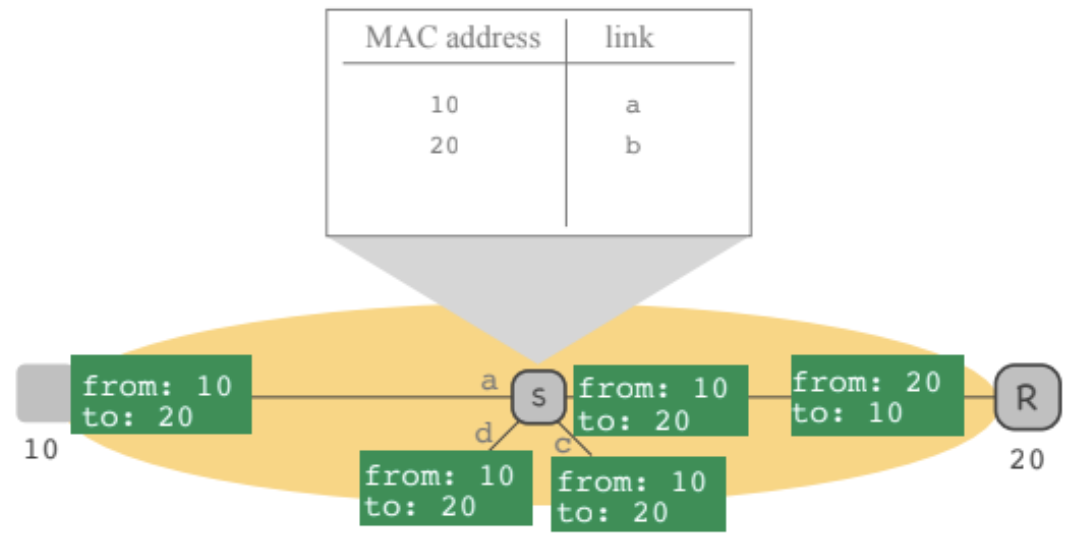
\includegraphics[width=0.7\textwidth]{images/link-layer-switch.png}
\end{center}

\subsubsection{Learning Algorithm}
\begin{enumerate}
    \item \textbf{Initial state:} Forwarding table is empty
    \item \textbf{Learning:} When a packet with source MAC address X arrives at link Y, add ``MAC X $\rightarrow$ link Y'' to the forwarding table
    \item \textbf{Unknown destinations:} When a packet arrives with unknown destination MAC, broadcast it to all links
\end{enumerate}

The figure above illustrates this process: when the switch receives a packet from MAC address 10 on link a, it learns that MAC 10 is reachable via link a. Similarly, when it receives traffic from MAC 20 on link b, it updates its forwarding table accordingly.

\subsubsection{Learning vs Routing Comparison}

\begin{description}
    \item[L2 Learning:] Passive learning from actual traffic; no explicit control messages
    \item[IP Routing:] Active exchange of routing protocol messages between routers
\end{description}

\subsubsection{The Broadcasting Problem: Forwarding Loops}

Broadcasting unknown destinations creates a serious problem: \textbf{forwarding loops}. If switches naively broadcast to all links, packets can circulate forever in network loops.

\textbf{Spanning Tree Solution:}

To prevent loops, switches use the \textbf{Spanning Tree Protocol}:

\begin{itemize}
    \item Creates a loop-free subgraph connecting all devices
    \item Includes all nodes but only a subset of links
    \item Broadcasts propagate only along tree edges
    \item Eliminates forwarding loops while maintaining connectivity
\end{itemize}

A spanning tree includes just enough links to reach every device without creating cycles---you cannot remove any edge without disconnecting some node.

\subsection{Address Resolution Protocol (ARP)}

We've explained how switches forward packets using MAC addresses, but a crucial question remains: \textbf{How does a device determine the MAC address of its intended recipient?} This is where the Address Resolution Protocol (ARP) comes in.

\subsubsection{The Problem: IP to MAC Address Mapping}

When Alice wants to send a packet, she faces two requirements:
\begin{enumerate}
    \item \textbf{Destination IP address:} Obtained from DNS (e.g., Bob's IP address)
    \item \textbf{Destination MAC address:} Unknown---this is what ARP solves
\end{enumerate}

\subsubsection{Scenario 1: Same Subnet Communication}

When Alice wants to send a packet to Bob in the same IP subnet:

\begin{enumerate}
    \item \textbf{ARP Request:} Alice broadcasts a request asking ``Who has IP address 128.178.2.20? Tell 128.178.2.10 (Alice's IP)''
    \item \textbf{Broadcasting:} Request uses special broadcast MAC address \texttt{FF-FF-FF-FF-FF-FF}, reaching every device in the subnet
    \item \textbf{ARP Response:} Bob recognizes his IP address and responds directly to Alice with his MAC address
    \item \textbf{Communication:} Alice now knows Bob's MAC address and can send packets directly
\end{enumerate}

\subsubsection{Scenario 2: Different Subnet Communication}

When Alice wants to send a packet to Bob in a different IP subnet:

\begin{enumerate}
    \item \textbf{Default Gateway:} Alice knows her router's IP address (e.g., 128.178.2.1) through configuration
    \item \textbf{ARP Request:} Alice broadcasts asking for the router's MAC address
    \item \textbf{Router Response:} Router responds with its MAC address
    \item \textbf{Packet Forwarding:} Alice sends packets to Bob using the router's MAC address as destination
\end{enumerate}

\subsubsection{ARP vs DNS Comparison}

\begin{description}
    \item[ARP:] Uses broadcasting within local subnet; no centralized infrastructure; each device knows its own MAC address
    \item[DNS:] Uses hierarchical server infrastructure; logically centralized mapping; dedicated servers maintain databases
\end{description}

Both serve address resolution roles but operate at different scales and use different mechanisms.

\section{Design Trade-offs and Architecture}

\subsection{Could We Eliminate IP Addresses?}

An interesting question: Could the entire Internet be one big Ethernet subnet using only MAC addresses?

\textbf{Answer: No, this wouldn't scale.}

\begin{itemize}
    \item \textbf{Forwarding table explosion:} Switches would need individual entries for millions of active devices
    \item \textbf{Broadcasting chaos:} Every address resolution would broadcast to the entire Internet
    \item \textbf{No aggregation:} Flat MAC addresses prevent the hierarchical aggregation that makes IP routing scalable
\end{itemize}

\subsection{Could We Eliminate MAC Addresses?}

Alternatively: Could we use only IP addresses and routers everywhere?

\textbf{Answer: Yes, this would scale, but we'd lose flexibility.}

The Internet was designed as a \emph{network of networks}---different types of subnets (Ethernet, WiFi, fiber, etc.) interconnected by IP routers. Eliminating the link layer would require replacing all specialized network equipment with IP routers, reducing the diversity and adaptability that make the Internet robust.

\subsection{Ethernet Elements Summary}

The complete Ethernet system relies on three core components:

\begin{description}
    \item[Address Resolution Protocol:] Maps IP addresses to MAC addresses (analogous to DNS)
    \item[L2 Forwarding:] Routes packets based on flat MAC addresses (analogous to IP forwarding)
    \item[L2 Learning:] Populates switch forwarding tables (analogous to IP routing protocols)
\end{description}

\newpage
\section{Complete Example: Packet Journey}

Now let's trace through a complete example showing how all these pieces work together when Alice sends a DNS request to access a web server:

\begin{center}
    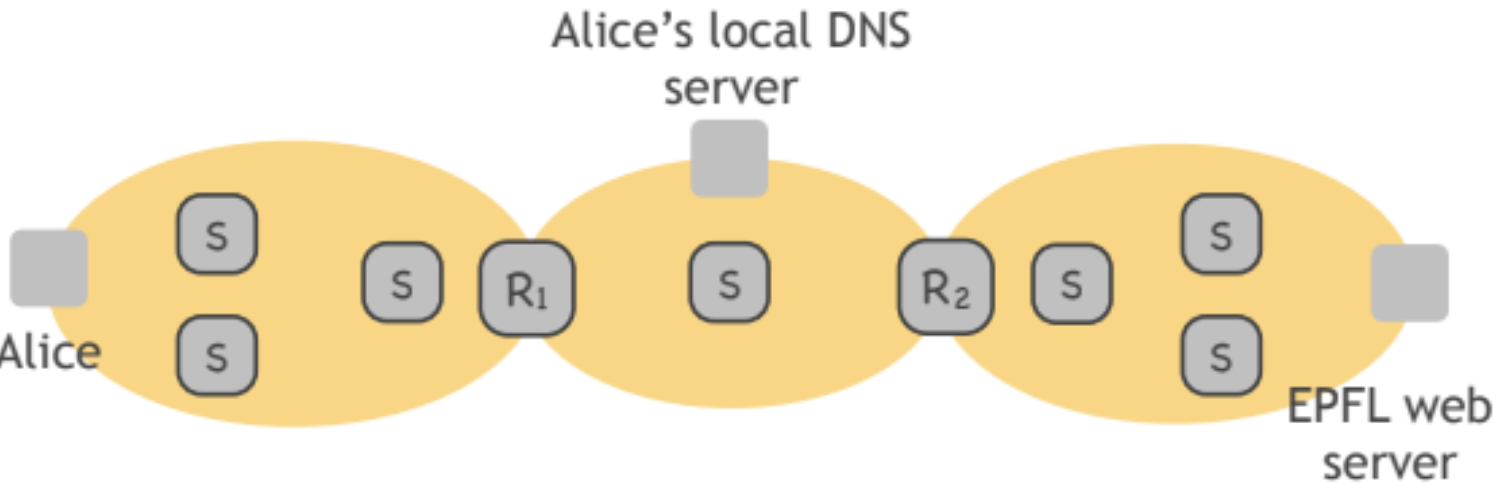
\includegraphics[width=0.8\textwidth]{images/topology-example.png}
\end{center}

\subsection{The Scenario}

When Alice types \texttt{http://www.epfl.ch} in her browser, this generates at least four packets:
\begin{enumerate}
    \item Alice's DNS request to local DNS server
    \item Local DNS server's response to Alice  
    \item Alice's HTTP GET request to web server
    \item Web server's response to Alice
\end{enumerate}

We'll focus on the first packet: Alice's DNS request to her local DNS server.

\subsection{Step-by-Step Packet Journey}

\subsubsection{Step 1: Application Layer Creates DNS Request}
Alice's DNS client process creates a DNS request to resolve \texttt{www.epfl.ch}, which is passed down to the transport and network layers:
\begin{itemize}
    \item \textbf{Source IP:} Alice's IP address
    \item \textbf{Destination IP:} Local DNS server's IP address (known via configuration)
\end{itemize}

\subsubsection{Step 2: ARP Request for Local Router}
Alice's network layer needs to determine the appropriate destination MAC address. Since the DNS server is in a different subnet, Alice must send the packet to her default gateway (router R1). She broadcasts an ARP request to resolve the router's IP address to its MAC address.

\subsubsection{Step 3: ARP Response from Router}
Router R1 receives the ARP request, recognizes its own IP address, and responds with its MAC address.

\subsubsection{Step 4: DNS Request with MAC Headers}
Alice can now send the DNS request with proper addressing:
\begin{itemize}
    \item \textbf{Source MAC:} Alice's MAC address
    \item \textbf{Destination MAC:} R1's MAC address
    \item \textbf{Source IP:} Alice's IP address  
    \item \textbf{Destination IP:} DNS server's IP address
\end{itemize}

\subsubsection{Step 5: Router Performs IP Forwarding}
R1 receives the packet, examines the destination IP address, and consults its forwarding table to determine the next hop toward the DNS server.

\subsubsection{Step 6: Router's ARP Request}
R1 needs to forward the packet to the next subnet containing the DNS server. It broadcasts an ARP request to resolve the DNS server's IP address to its MAC address.

\subsubsection{Step 7: DNS Server's ARP Response}
The DNS server receives the ARP request and responds with its MAC address.

\subsubsection{Step 8: Final Packet Delivery}
R1 forwards the DNS request with updated MAC addresses:
\begin{itemize}
    \item \textbf{Source MAC:} R1's MAC address (in the new subnet)
    \item \textbf{Destination MAC:} DNS server's MAC address
    \item \textbf{Source IP:} Alice's IP address (unchanged)
    \item \textbf{Destination IP:} DNS server's IP address (unchanged)
\end{itemize}

\subsubsection{Address Requirements}
\begin{itemize}
    \item \textbf{End-systems and routers need MAC addresses:} Otherwise, switches wouldn't know where to forward packets within subnets
    \item \textbf{End-systems need IP addresses:} Otherwise, routers wouldn't know where to forward packets across the Internet
    \item \textbf{Switches don't need MAC addresses for forwarding:} They learn MAC-to-port mappings automatically
    \item \textbf{Routers don't need IP addresses for forwarding:} They use destination IP addresses in packet headers
\end{itemize}

\newpage
\section{Network Hierarchy Summary}

The Internet operates at three distinct levels, each with its own addressing and routing mechanisms:

\subsection{Level 1: IP Subnets}
\begin{itemize}
    \item \textbf{Devices:} Link-layer switches connecting end-systems and routers
    \item \textbf{Forwarding:} L2 forwarding based on MAC addresses
    \item \textbf{Learning:} L2 learning populates switch forwarding tables automatically
\end{itemize}

\subsection{Level 2: Autonomous Systems (AS)}
\begin{itemize}
    \item \textbf{Devices:} IP routers connecting multiple IP subnets within one administrative domain
    \item \textbf{Forwarding:} IP (L3) forwarding based on IP addresses
    \item \textbf{Routing:} Intra-domain routing protocols (OSPF, RIP) populate router forwarding tables
\end{itemize}

\subsection{Level 3: Internet}
\begin{itemize}
    \item \textbf{Devices:} Border routers connecting multiple Autonomous Systems
    \item \textbf{Forwarding:} IP (L3) forwarding based on IP addresses
    \item \textbf{Routing:} Inter-domain routing protocol (BGP) coordinates between ASes
\end{itemize}

Each level uses appropriate addressing schemes and protocols optimized for its scale and administrative requirements, creating a hierarchical system that enables the Internet's remarkable scalability and robustness.

\end{document}